\section{Ausgangssituation}\label{sec: initial_situation}

Es gibt bereits viele VR Applikation, aber was ist genau eine VR Applikation.
Es gibt viele Definitionen für VR ausgeschrieben Virtual Reality.
In dieser Arbeit sprechen wir über die Wirklichkeit welche durch ein head mounted display, oder umgangssprachlich auch eine VR-Brille angezeigt wird.
Somit bezeichnet eine VR Application eine Software, welche in der VR-Brille läuft.

Von diesen VR Applikationen gibt es schon einige.
Die meisten werden im Bereich Videospiele verwendet nach einer Statistik aus Deutschland im Jahre 2021, bei welcher Personen mit einer VR-Brille oder head mounted display befragt worden sind.
Siehe Abbildung~\ref{fig:statistic_usage_vr}~\cite{BITKOM_2021}

\begin{figure}
    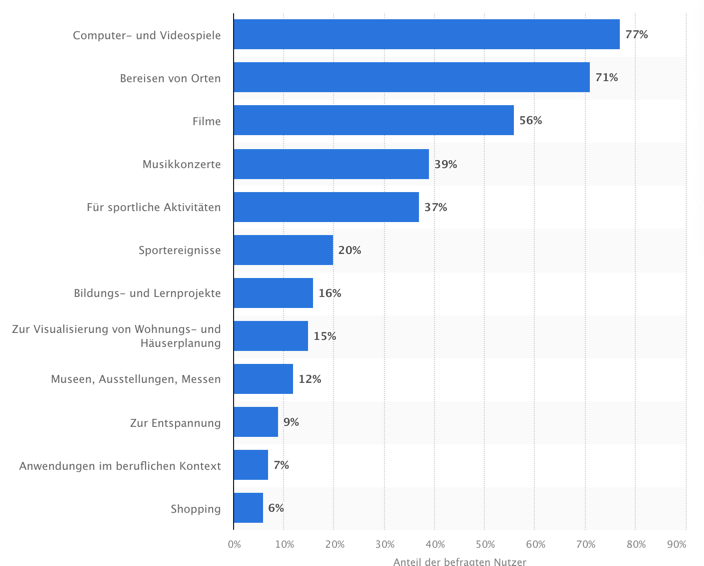
\includegraphics[scale=0.5]{pics/statistic_usage_vr}
    \caption{Anwendungsgebiete VR}
    \label{fig:statistic_usage_vr}
\end{figure}

Bei diesen VR Applikationen ist meist der Kopf getrackt und vielleicht auch Hände, Füße und Hüften.
Interconversions sind meistens aber die weitere interaktion mit der Umgebung.
Setzt einer sich auf einen Sessel wird er durchfliegen, außer er steht auch in der realen Wirklichkeit dort.

\section{Zielsetzung}\label{sec: objective}

Das Ziel von Beam VR ist die physische Realität und die virtuelle Realität zu kombinieren.
Im Falle Beam VR benützen wir hier einen Balken, welcher von einem Hochhaus wegsteht.
Dieser Balken soll in der physischen Realität und in der virtuellen Realität existieren und die gleiche Position einehmen.
Dadurch soll die Immersion entstehen, dass man wirklich auf einem Balken steht, welcher von einem Hochhaus wegsteht.
Auch, wenn man nur in seinem Wohnzimmer oder auch woanders ohne Gefahren auf einem Balken steht.
Beam VR ist nicht der Erfinder dieses Konzeptes.
Mehr dazu gibt es in der kommenden Umfeldanalyse.

